\documentclass{beamer}
\usepackage{beamerthemesplit}
\usepackage{graphics}
\logo{
\includegraphics[height=1cm]{psi_logo_white.png}}
\usetheme{Pittsburgh}
\usecolortheme{dove}
\beamertemplatenavigationsymbolsempty
\setbeamertemplate{footline}[frame number]
\definecolor{myback}{RGB}{175,238,238}
\setbeamercolor{structure}{bg=myback}
\usepackage[T1]{fontenc}
\newcommand{\changefont}[3] {
 \fontfamily{#1} \fontseries{#2} \fontshape{#3} \selectfont}

\title{NeXus Recapitulation and Developments}
\author{Mark K\"onnecke }
\institute{NeXus International Advisory Committee}
\date{\today} 

\begin{document}

\begin{frame}
\titlepage
\end{frame}

\begin{frame}
\frametitle{Table Of Content}
\begin{itemize}
\item Brief Introduction to NeXus
\item Decisions from NIAC 2010
\item Developments since NIAC 2010
\item Topics for this NIAC Meeting
\end{itemize}
\end{frame}


\begin{frame} \frametitle{NeXus Mission}
\begin{itemize}
\item Definition of a standard data format
\begin{itemize}
\item Rules
\item Validation tools
\end{itemize}
\item Promotion of NeXus
\begin{itemize}
\item Documentation
\item NeXus API
\item Outreach to the scientific community
\end{itemize}
\end{itemize}
\end{frame}

\begin{frame} \frametitle{NeXus Design}
\begin{itemize}
\item Complete data for typical use
\item Extendable, add additional data as you please
\item Self describing
\item Easy automatic plotting
\item Store a full beamline description (FBD)
\item Platform independent, public domain, efficient
\item Suitable for a wild variety of applications
\end{itemize}
\end{frame}

\begin{frame}
 \frametitle{NeXus Levels }
\begin{enumerate}
\item Physical file format and API for accessing files
\item Rules for storing data in files
\item Component and application definitions
\item NeXus Utilities
\end{enumerate}
\end{frame}

\begin{frame}
\frametitle{Decisions from NIAC 2010}
\begin{itemize}
\item NXsubentry
\item NXcollection
\item Support for CIF style coordinate systems
\item Non C-storage order arrays: offset, stride attributes
\item Python tree API becomes part of NAPI
\item Look into NAPI thread safety and PHDF
\end{itemize}
\end{frame}

\begin{frame} \frametitle{NXsubentry}
\begin{tabbing}
\hspace*{1cm} \= \hspace*{1cm} \= \hspace*{1cm} \= \hspace*{1cm} \= \hspace*{1cm} \= \hspace*{1cm}\= \kill
entry:NXentry \\
\>sample:NXsample\\
\>instrument:NXinstrument\\
\>.....\\
 \>sas:NXsubentry\\
 \>  \>sample:NXsample \\
\\
\> \>instrument:NXinstrument\\
\> \> \> source:NXsource\\
\> \> \> velocity\_selector:NXvelocity\_selector\\
\> \> \> detector:NXdetector \\
\> \> \> \>data[xsize,ysize], signal=1 (1)\\
\> \>control:NXmonitor\\
\> \> \>data\\
\> \>data:NXdata\\
\> \> \> link to (1)\\
\end{tabbing}
\end{frame}

\begin{frame} \frametitle{NXcollection}
\begin{tabbing}
\hspace*{1cm} \= \hspace*{1cm} \= \hspace*{1cm} \= \hspace*{1cm} \= \hspace*{1cm} \= \hspace*{1cm}\= \kill
\>entry,NXentry\\
\> \>measurement:NXcollection\\
\> \> \>positions:NXcollection\\
\> \> \> \>om \\
\> \> \> \>two\_theta\\
\> \> \>scalars:NXcollection\\
\> \> \> \>title\\
\> \> \> \>wavelength\\
\> \> \>data:NXdata\\
\> \> \> \>detector1\\
\> \> \> \>mca5\\
\end{tabbing}
\end{frame}


\begin{frame}
\frametitle{Developments since 2010}
\begin{itemize}
\item HDRI Meeting Hamburg
\item PanData floundered
\item Code Camp 2011
\item Collaboration with DECTRIS
\item Code Camp 2012
\item NAPI release 4.3, NXDL 3.2 == 1.0
\end{itemize}
\end{frame}


\begin{frame}
\frametitle{HDRI: High Data Rate Initiative}
\begin{itemize}
\item German synchrotron and neutron sources 
\item Collaboration with little money
\item Invented something NeXus alike
\item Later convinced to go NeXus
\item Additional and revised synchrotron base classes
\begin{itemize}
\item NXcapillary
\item NXbending\_magnet
\item NXinsertion\_device
\item NXxray\_lens
\end{itemize}
\item Current state: Eugen?
\end{itemize}
\end{frame}


\begin{frame}
\frametitle{PanData}
\begin{itemize}
\item European project to standardize logins, data catalogs and data
\item NeXus at first well received
\item Then plans to develop method specific formats between facilities
\item Dormant ever since
\end{itemize}
\end{frame}


\begin{frame}
\frametitle{Code Camp 2011}
\begin{itemize}
\item At APS 
\item NX\_UNLIMITED for all dimensions
\item 64 bit dimensions
\item HDF-5 1.8
\item Documentation updates
\item WWW-site from manual
\item NXimpatient dodument: NeXus in 8 pages
\item Test for python-API 30\% complete
\item Python Tree API cleaned up
\item PHDF not useful
\item New C++ Tree API (Eugen)
\end{itemize}
\end{frame}


\begin{frame}
\frametitle{Collaboration with DECTRIS}
\begin{itemize}
\item Manufacturer of Pilatus and Eiger detectors
\item Going for NeXus/HDF-5 for Eiger
\item Detector Software writes NXdetector group
\item More fields added to NXdetector to accomodate pixel detectors
\item This is well on its way
\end{itemize}
\end{frame}

\begin{frame} \frametitle{DECTRIS File Structure}
\begin{figure}[!ht]
\resizebox{7cm}{5cm}{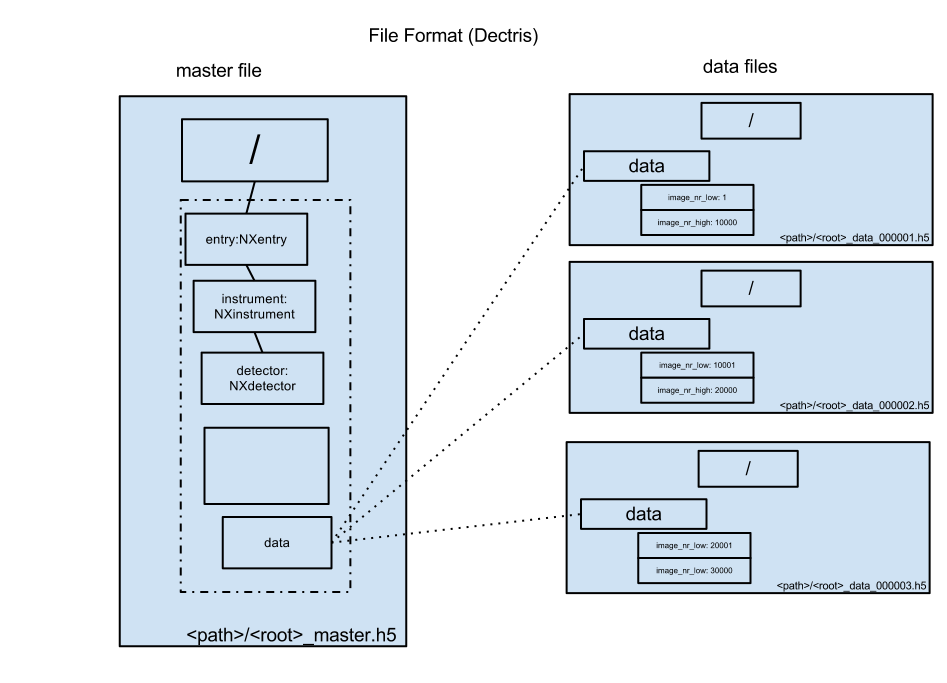
\includegraphics[width=0.75\textwidth]{HDF5-FileOrganisation.png}}\end{figure}
\end{frame}

\begin{frame}
\frametitle{Rationale}
\begin{itemize}
\item DECTRIS has a problem:
\begin{itemize}
\item Detector outputs 5-10 GB/sec
\item The deliver the detector and the computer going with it
\item They cannot ask their customers to provide the appropriate hardware for such 
 a detector: parallel file system etc.
\item Must compress and write the file on one computer
\item Compression has to be parallel as CPU intensive
\end{itemize}
\item File structure a workaround for HDF-5 not allowing sections of datsets in different 
 files
\item Sidenote: LZ4 or snappy compression; up to ~ 450MB/sec on write
\end{itemize}
\end{frame}


\begin{frame}
\frametitle{Upcoming DECTRIS Meeting with Community}
\begin{itemize}
\item DECTRIS aims at meeting customers in october
\item How far can we compromise?
\item Anyone from the NeXus community who wishes to join?
\item Comment from code camp: ask for tool to convert to HDF-5 standard compression
\end{itemize}
\end{frame}


\begin{frame}
\frametitle{HDF-5 Workshop at PSI}
\begin{itemize}
\item May 2012
\item Organised with DECTRIS to address performance issues
\item HDF people gave overview of new developments in HDF-5
\item DECTRIS (and DESY) pays for:
\begin{itemize}
\item Writing pre compressed chunks
\item Dynamically loadable filters
\end{itemize}
\end{itemize}
\end{frame}

\begin{frame}
\frametitle{New Feautures for HDF-5 1.10}
\begin{itemize}
\item Asynchronous I/O
\item Journaling
\item Single Writer, Multiple Reader semantics
\item Better fault tolerance
\item In memory HDF-5 files 
\item Shared object headers
\end{itemize}
\end{frame}

\begin{frame}
\frametitle{Other Things the HDF people work on}
\begin{itemize}
\item Better multi threading support
\item Virtual Object Layer, completely replace storage layer
\begin{itemize}
\item Use HDF-5 data model but not file format
\item Opens path to more storage models
\item Metadata server for better parallel support
\item Mirroring, stacking 
\end{itemize}
\item Better parallel processing support: meta data server
\end{itemize}
\end{frame}

\begin{frame}
\frametitle{NAPI Release 4.3, Application Definitions 3.1}
\begin{itemize}
\item 64 bit dimensions
\item HDF-1.8
\item NX\_UNLIMITED everywhere
\item Alpha python tree API included
\item First release of applicaton definitions
\item Updated manual
\end{itemize}
\end{frame}


\begin{frame}
\frametitle{Code Camp 2012}
\begin{itemize}
\item Moved documentation to sphinx
\begin{itemize}
\item Wiki like syntax allows for easier editing then docbook
\item URL: 
\end{itemize}
\item Cleaned up trac tickets
\item Decided to drop autoconf in favour of CMake
\item Resolved CIF coordinate issue
\item Devised a good suggestion for handling axes at multidimensional 
  datasets
\item Cleanup of NeXus applications: nx2dtd, NXDump, nxtraverse, NXformat\_dfn dropped
\item Got NAPI 4.3 release ready
\end{itemize}
\end{frame}


\begin{frame}
\frametitle{Topics for NIAC 2012}
\begin{itemize}
\item Review of NeXus: where are we headed?
\item Roadmap OO-NeXus
\item CIF coordinates
\item Process for changing base classes
\item Review synchrotron beamline classes
\item Review additions to NXdetector
\item Materials definition
\item Multi dimensional array axes encoding
\item What to do about expired NIAC members?
\item Electing new officers
\end{itemize}
\end{frame}

\begin{frame}
\frametitle{Questions from Code Camp}
\begin{itemize}
\item Is anyone using NXcharacterization? Remove?
\item Who is using F77 NAPI? How much effort to put into this?
\item Do we go into timed data?
\end{itemize}
\end{frame}


\begin{frame}
\frametitle{CIF Revisited}
\begin{itemize}
\item Finalize
\item Hope for endorsement of CIF community
\item AIM: provide data necessary to derive positions of components from 
 transformation matrics
\end{itemize}
\end{frame}

\begin{frame} \frametitle{Transformation Matrices}
\begin{math}
T = \left( \begin{array}{cccc}
1 & 0 & 0 & x\\
0 & 1 & 0 & y\\
0 & 0 & 1 & z\\
0 & 0 & 0 & 1\\
\end{array} \right)
\end{math}

\begin{math}
\onslide+<2-> 
R = \left( \begin{array}{cccc}
r11 & r12 & r13 & 0\\
r21 & r22 & r23 & 0\\
r31 & r32 & r33 & 0\\
0 & 0 & 0 & 1\\
\end{array} \right)
\end{math}

\end{frame}

\begin{frame} \frametitle{Combining Transformations}
\begin{figure}[!ht]
\resizebox{7cm}{5cm}{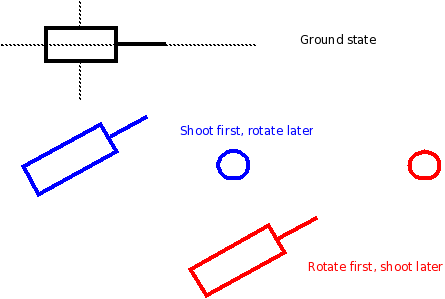
\includegraphics[width=0.75\textwidth]{rotcombi.png}}\end{figure}
\end{frame}

\begin{frame} \frametitle{Some Properties}
\begin{itemize}
\item Transformations can be combined by matrix multiplications
\item Individual matrices can be derived by looking at the situation when everything else is 0
\item Absolute positions can be obtained by multiplying the resulting matrix with its transpose
\item Defines new coordinate systems at components
\item CIF contains a duplication: vector, offset scheme 
\end{itemize}
\end{frame}

\begin{frame} \frametitle{What Use Is This?}
\begin{itemize}
\item Allows to calculate absolute positions of components in the laboratory coordinate systems
\item Can directly convert from a detector coordinate system to  
 vectors in Lab coordinate system
\item Calculate things like impact of primary beam on detector, SAS
\item Allows arbitray axis to be expressed
\item Intuitively describe an instrument with angles and translations and still be able
 to recover absolute coordinates
\end{itemize}
\end{frame}


\begin{frame} \frametitle{NeXus Axis Mapped}
\begin{itemize}
\item rotation\_angle, polar\_angle, rotate 0 1 0
\item azimuthal\_angle, rotate 0 0 1
\item distance, translate 0 0  1
\item chi, rotate 0 0 1
\item phi rotate, 0 1 0
\item NeXus polar coordinate system: rotate azimuthal\_angle, rotate polar\_angle, 
 translate by distance
\end{itemize}
\end{frame}

\begin{frame} \frametitle{CIF Dependency Table}
\begin{tabular}{llllll}
axis-id &type &equipment&dependson &vector & offset\\
gonio\_phi &rotation& goniometer & . &1,0,0,& ...\\
det\_z&translation&detector& .& 0,0,-1& 0 0 0\\
det\_y&translation&detector&det\_z&0,1,0&0,0,0\\
det\_x&translation&detector&det\_y&1,0,0&0,0,0\\
\end{tabular}
\end{frame}


\begin{frame} \frametitle{Expressing Axis Dependency in NeXus}
\begin{itemize}
\item Implied: use existing NeXus coordinate system
\item dependson attribute pointing to depending axis
\item transform field in base classes which becomes a comma separated list of 
 the path to the transformations required to position this component
\item Create a special container to hold axis dependencies, NXdependency, to 
 collect the dependencies in one place for easy access. This is what CIF does
\end{itemize}
\end{frame}

\begin{frame} \frametitle{Dependons Option}
\begin{tabbing}
\hspace*{1cm} \= \hspace*{1cm} \= \hspace*{1cm} \= \hspace*{1cm} \= \hspace*{1cm} \= \hspace*{1cm}\= \kill
\>sample,NXsample\\
\> \>rotation\_angle\\
\> \>chi (dependson rotation\_angle)\\
\> \>phi (dependson phi)\\
\end{tabbing}
\end{frame}

\begin{frame} \frametitle{Transform Option}
\begin{tabbing}
\hspace*{1cm} \= \hspace*{1cm} \= \hspace*{1cm} \= \hspace*{1cm} \= \hspace*{1cm} \= \hspace*{1cm}\= \kill
\>sample,NXsample\\
\> \>rotation\_angle\\
\> \>chi \\
\> \>phi \\
\> \>transform = rotation\_angle,chi,phi \\
\end{tabbing}
\end{frame}


\begin{frame} \frametitle{Separate Group Option}
\begin{tabbing}
\hspace*{1cm} \= \hspace*{1cm} \= \hspace*{1cm} \= \hspace*{1cm} \= \hspace*{1cm} \= \hspace*{1cm}\= \kill
\>sample,NXsample\\
\> \>rotation\_angle\\
\> \>chi \\
\> \>phi \\
\>dependency,NXdependency\\
\> \>sample/chi = \\
\> \> \>sample/rotation\_angle\\
\> \>sample/phi =\\
\> \> \> sample/chi\\
\> \>instrument/detector/x\_translation = \\
\> \> \>instrument/detector/distance\\
\> \>instrument/detector/distance = \\
\> \> \>instrument/detector/polar\_angle\\
\end{tabbing}
\end{frame}

\begin{frame} \frametitle{Tech Committee Recommendation}
\begin{tabbing}
\hspace*{1cm} \= \hspace*{1cm} \= \hspace*{1cm} \= \hspace*{1cm} \= \hspace*{1cm} \= \hspace*{1cm}\= \kill
\>sample,NXsample\\
\> \>rotation\_angle (vector 0,1,0)\\
\> \>chi (depends\_on rotation\_angle, vector 0,0,1)\\
\> \>phi (depends\_on chi, vector 0,1,0)\\
\> \>depends\_on \\
\> \> \>phi \\
\end{tabbing}
\end{frame}

\begin{frame}
\frametitle{Tech Committe Recommendation Continued}
\begin{itemize}
\item Add offset attribute to fully cover CIF. This is an extra translation
\item offset\_unit to give units for offset
\item The vector attribute becomes mandatory
\item This gives us CIF endorsement! 
\end{itemize}
\end{frame}

\begin{frame}
\frametitle{Process for Adding Fields and Classes}
\begin{itemize}
\item Passing them through NIAC is slow (2 years!)
\item Must be documented well enough, no duplicates
\item Suggestion: leave to technical group
\item Suggestion2: technical group publishes changes to NIAC for intervention
\end{itemize}
\end{frame}

\begin{frame}
\frametitle{Review of Synchrotron Beamline Components}
\begin{itemize}
\item NXcapillary
\item NXbending\_magnet
\item NXinsertion\_device
\item NXxraylens
\end{itemize}
\end{frame}


\begin{frame}[fragile] 
\frametitle{NXdetector Additions for DECTRIS}
\begin{semiverbatim}
  acquisition\_mode:NX\_CHAR
  angular\_calibration:NX\_FLOAT[i,j]
  angular\_calibration\_applied:NX\_BOOLEAN
  bit\_depth\_readout:NX\_INT
  countrate\_correction\_\_applied:NX\_BOOLEAN
  countrate\_correction:NX\_FLOAT[i,j]
  detector\_readout\_time:NX\_FLOAT
  exposure\_time\_time:NX\_FLOAT
  flatfield:NX\_FLOAT[i,j]
  flatfield\_applied:NX\_BOOLEAN
  flatfield\_error:NX\_FLOAT[i,j]
  frame\_start\_number:NX\_INT
  frame\_time:NX\_FLOAT[NP]
\end{semiverbatim}
\end{frame}

\begin{frame}[fragile] 
\frametitle{NXdetector Additions for DECTRIS 2}
\begin{semiverbatim}
  gain\_setting:NX\_CHAR
  pixel\_mask:NX\_FLOAT[i,j]
  pixel\_mask\_applied:NX\_BOOLEAN
  saturation\_value:NX\_INT
  sensor\_material:NX\_CHAR
  sensor\_thickness:NX\_FLOAT
  threshold\_energy:NX\_FLOAT
  trigger\_dead\_time:NX\_FLOAT
  trigger\_delay\_time:NX\_FLOAT
\end{semiverbatim}
\end{frame}

\begin{frame}
\frametitle{Materials Definition Recommendation}
\begin{itemize}
\item This is about defining materials: samples, filters, multi layers etc. 
\item Bag of worms
\item Recommendation
\begin{itemize}
\item Use textual description
\item When decisive for DA: community should suggest enums
\end{itemize}
\end{itemize}
\end{frame}

\begin{frame}
\frametitle{Time Based Data}
\begin{itemize}
\item Neutron event data to be correlated with other time based data
\item Dynamic scans collecting detector frames and other data with possibly 
  different sampling rates
\item FELS will collect data only dynamically
\item We have NXlog
\item Questions to the NIAC:
\begin{itemize}
\item Shall NeXus expand into this market?
\item Is the tech committee to be tasked to develop a recommendation how to store this 
  better?
\end{itemize}
\end{itemize}
\end{frame}

\end{document}






\begin{frame}
\frametitle{}
\begin{itemize}
\item
\item
\item
\item
\end{itemize}
\end{frame}

\begin{frame}
\frametitle{The Predicament of the Traveling Scientist}
\begin{itemize}
\item<1->A different data format wherever she goes
\item<2->Spends lots of time converting formats or writing readers
\item<3->Waits even longer to load data from inefficient data formats
\item<4->DA requires N files in different  formats, notes, local knowledge 
\item<5->Cannot read her collaborators data
\item<6->Has to keep extra information in yet another form
\end{itemize}
\end{frame}


\begin{frame} \frametitle{Conclusion }
\begin{itemize}
\item NeXus is a mature and capable data format
\item There is no other standard then NeXus on the horizon
\item New things are developed with NeXus everywhere, uptake at established sites is slow
\item You are invited to join the NIAC and contribute to NeXus 
\item More information: http://www.nexusformat.org (outdated, but working on it)
\end{itemize}
\end{frame}


\begin{frame} \frametitle{Example Files}
\end{frame}

\begin{frame} \frametitle{Storing Single Data Items }
\begin{itemize}\item Units have to specified
\item Locating axis, by example:
\begin{itemize}\item counts(two\_theta, time\_of\_flight), attributes: signal=1
\item two\_theta, attributes: axis=1, axis=primary 
\item time\_of\_fligth, attributes: axis=2, axis=primary
\end{itemize}\end{itemize}
\end{frame}

\begin{frame} \frametitle{NXtranslate }
\begin{itemize}\item Anything to NeXus converter:
\begin{itemize}\item Binary dump
\item FRM2
\item IPNS run
\item NeXus
\item Spec
\item XML
\end{itemize}\item Uses XML based translation file to control translation
\item Extendable via plugins
\end{itemize}
\end{frame}

\begin{frame} \frametitle{NXextract}
\begin{itemize}
\item Extracts NeXus files to binary or ASCII
\item Uses XML template file to control conversion
\item Contributed by Stephane Poirier, SOLEIL 
\end{itemize}
\end{frame}

\begin{frame} \frametitle{Another Way to use NeXus/HDF-5}
\begin{enumerate}
\item Use NXopenpath(hfil,path) to access the data in file, use introspection to 
 find out about dimensions
\item Have a dictionary mapping what you need for DA to paths
\item Keep the dictionary in a separate file
\item When you encounter a different file, just edit the dictionary file 
\end{enumerate}
\end{frame}

\begin{frame} \frametitle{McStas Coordinate System }
\begin{figure}[!ht]
\resizebox{7cm}{5cm}{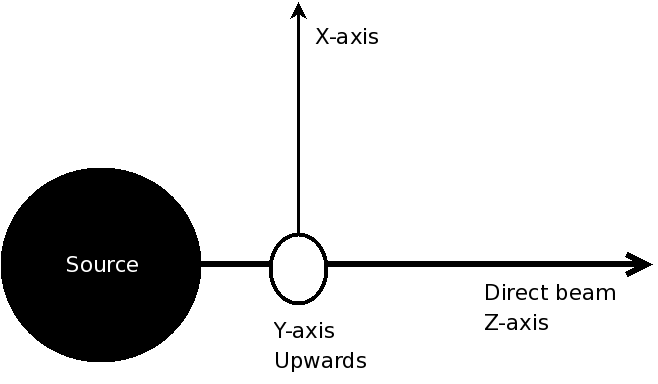
\includegraphics[width=0.75\textwidth]{mcstas.png}}\end{figure}
\end{frame}

\begin{frame} \frametitle{NeXus Simple Coordinate System }
\begin{figure}[!ht]
\resizebox{7cm}{5cm}{\includegraphics[width=0.75\textwidth]{polplane.png}}\end{figure}
\end{frame}




\begin{frame} 
\frametitle{NeXus Endorsement }
\begin{table}[!ht]
\begin{tabular}{|c|c|c|}
\hline
SNS at ORNL & SINQ at PSI\\ \hline
 NCNR at NIST & ISIS at RAL\\ \hline
 Diamond at RAL&Opal at ANSTO\\ \hline
FRM2 at TUM&KENS at KEK\\ \hline
J-Parc & IPNS at ANL\\ \hline
APS at ANL& HMI in Berlin\\ \hline
MLNSC at LANL& LLB in Saclay\\ \hline
\end{tabular}\end{table}
\end{frame}




\begin{frame} \frametitle{NeXus Levels }
\begin{enumerate}\item Physical file format
\item API for accessing files
\item Structure for organizing data in files
\item Rules for storing individual data items
\item Component and application definitions
\end{enumerate}
\end{frame}

\begin{frame} \frametitle{NXtranslate }
\begin{itemize}\item Anything to NeXus converter:
\begin{itemize}\item Binary dump
\item FRM2
\item IPNS run
\item NeXus
\item Spec
\item XML
\end{itemize}\item Uses XML based translation file to control translation
\item Extendable via plugins
\end{itemize}
\end{frame}

\begin{frame} \frametitle{NXextract}
\begin{itemize}
\item Extracts NeXus files to binary or ASCII
\item Uses XML template file to control conversion
\item Contributed by Stephane Poirier, SOLEIL 
\end{itemize}
\end{frame}


\begin{frame}[fragile] 
\frametitle{Aside: CIF Hierarchies}
CIF uses Hierarchies too, but hides them:
\uncover<1->{
\begin{semiverbatim}
\_exptl\_crystal\_description        plate\newline
\_exptl\_crystal\_colour             colourless\newline
\_exptl\_crystal\_size\_max           0.30
\end{semiverbatim}
}
\uncover<2>{
\begin{semiverbatim}
/exptl/crystal/description        plate\newline
/exptl/crystal/colour             colourless\newline
/exptl/crystal/size/max           0.30
\end{semiverbatim}
}

\end{frame}

\begin{frame}
\frametitle{Why a Common Dataformat? }

\begin{itemize}\item Today: 
\begin{itemize}\item Lots of different data formats
\item Time wasted converting data
\item Old formats no longer capable of delivering for new high throughput detectors
\item Difficult to add additional data
\item Often, for DA multiple different files needed
\item Badly documented formats
\end{itemize}\item Tomorrow, with NeXus:
\begin{itemize}
\item Single, efficient, platform independent data format
\item All information in one file
\item Self describing
\item Extendable
\end{itemize}
\end{itemize}
\end{frame}

\begin{frame} \frametitle{Using Tabbing for Hierarchy}
\begin{tabbing}
\hspace*{1cm} \= \hspace*{1cm} \= \hspace*{1cm} \= \hspace*{1cm} \= \kill
entry:NXentry \\
 \>sample:NXsample \\
 \> \> rotation\_angle[NP], axis=1 (1) \\
\\
 \>instrument:NXinstrument\\
 \> \> detector:NXdetector \\
 \> \> \>data[NP], signal=1 (2)\\
 \>data:NXdata\\
 \> \> link to (1)\\
 \> \> link to (2)\\
\end{tabbing}
\end{frame}
